\subsection{Level2.3: $y=-x*sin(x)$ について}
この関数はいくつかの峰と谷を持つ複雑な関数であり,谷を見つけてもそこが最低値かどうかは判断出来ない.そこで以下のようのソースコードを修正した.
\subsubsection{プログラムソース(変更部分)}
\begin{lstlisting}[caption=変更部分,label=fix01]
--------------...
83     n=4;
84     d=X_RANGE/n;
85
86     for (j=0; j < n;j++){
87       x = X_MIN+d*j + (X_RANGE/n) * (double)rand()/RAND_MAX;
...------------
\end{lstlisting}
\subsubsection{観察意図と観察方法}
 これは,最急降下法で観察する部分を分割することで,様々な場所の最小値を発見しようとしている.変更したのは初期値だけであるが,最急降下法は初期値の発生位置によって結果が大きく左右されるため十分であると判断した.観察は当初出力結果を観察していたが,データの推移が判断しにくいためgnuplotでのグラフとの比較を見て判断した.グラフの作成にはシェルスクリプト(スクリプト2.3参照)を用いた.
\subsubsection{実行結果}

\begin{figure}[htb]
 \begin{center}
 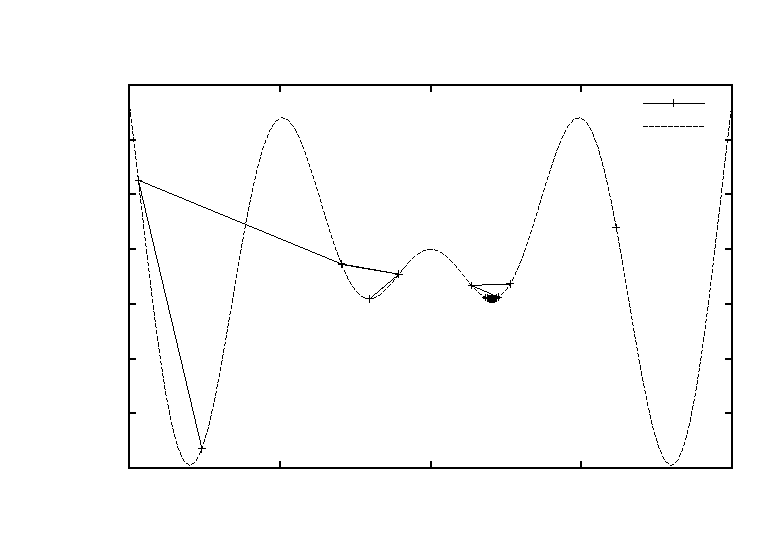
\includegraphics[width=10.0cm]{./level2/level2.3.eps}
  \caption{修正されたプログラムによる出力結果}
  \label{level2.3}
 \end{center}
\end{figure}
\subsubsection{考察}
上の結果が示すように分割した位置で最急降下法を実行することにより,それぞれの谷の位置を発見することが出来た.今回は谷の数を考慮したn(分割数)=4でプログラムを実行したが,現実的にはnもパラメータとして定義し,都合の良い値を推測べきである.

